\documentclass[conference]{IEEEtran}
\usepackage{amsmath,amssymb,amsfonts}
\usepackage{graphicx}
\usepackage{textcomp}
\usepackage{xcolor}
\usepackage{booktabs}
\usepackage{multirow}
\usepackage{cite}
\usepackage{url}
\usepackage{microtype}

\graphicspath{{figures/}}

\begin{document}

\title{Introduction to Artificial Intelligence}

\author{
    \IEEEauthorblockN{Ho\`ang Xu\^an Th\`anh}
    \IEEEauthorblockA{523h0178@student.tdtu.edu.vn}
    \and
    \IEEEauthorblockN{Nguy\~{\^e}n L\^e Ph\'u Huy}
    \IEEEauthorblockA{524h0090@student.tdtu.edu.vn}
    \and
    \IEEEauthorblockN{Nguy\~{\^e}n Th\`anh An, M.Sc.}
    \IEEEauthorblockA{nguyenthanhan@tdtu.edu.vn}
}

\maketitle

\begin{abstract}
This report presents our complete solution for the Final Project in Introduction to Artificial Intelligence (Course 503043). We address all four stated project requirements across three distinct AI search paradigms:
(1) For the $N$-Queens problem, we formulate the domain under Propositional Logic via an $O(N^2)$ constraint discovery algorithm and Conjunctive Normal Form (CNF) conversion with closed-form clause bound $\Theta(N^3)$, solved with Glucose3 (PySAT); we additionally implement Min-Conflicts local search and propose a ``Most-Conflicted with Tabu Tenure'' heuristic that reduces median iterations to 56\%--76\% across board sizes up to $N=1000$.
(2) For Tank Battle, we formulate a 2-player zero-sum game with alternating 2-ply cycle abstractions; on 10 terminal endgame positions, exact $\alpha$-$\beta$ pruning reduces explored nodes by up to $114\times$ (cutting effective branching factor $b^*$ from 5.36 to 2.89) while preserving identical minimax values; for real-time play, depth-limited Heuristic $\alpha$-$\beta$ with Transposition Table caching and vectorized move ordering slashes explored nodes by 64.4\%--85.9\%, executing depth 4 (8 plies) in 8.65~ms and depth 5 (10 plies) in 22.04~ms, remaining undefeated in tournament play.
(3) For Kakuro puzzles, we formulate a high-arity Constraint Satisfaction Problem (CSP) and enforce Generalized Arc Consistency (GAC) using Kuhn's bipartite matching algorithm integrated into Backtracking Search; initial AC-3 preprocessing deterministically shrinks the search space from $10^{45.8}$ to $1$, solving the complex $9 \times 9$ (48-variable) benchmark with 0 backtracks in 9.1~ms and completely eliminating heavy-tailed search variance.
All functional requirements, experimental benchmarks, unit test suites, and interactive graphical environments are 100\% completed and verified.
\end{abstract}

\begin{IEEEkeywords}
Propositional Logic, SAT Solver, Min-Conflicts, Adversarial Search, Minimax, Alpha-Beta Pruning, Constraint Satisfaction Problems, Kakuro, Arc Consistency.
\end{IEEEkeywords}

\section{Introduction}
Search algorithms form the core foundation of classic Artificial Intelligence. Depending on the problem environment, agents must reason under deterministic constraints, navigate competitive multi-agent dynamics, or optimize combinatorial assignments. This project explores three critical paradigms:
\begin{enumerate}
    \item \textbf{Logic and Local Search:} Encoding $N$-Queens into Conjunctive Normal Form (CNF) for CDCL SAT solvers, alongside an adaptive local search heuristic.
    \item \textbf{Adversarial Search:} Modeling simultaneous discrete combat into an alternating zero-sum game with game-tree search and domain-specific heuristics.
    \item \textbf{Constraint Satisfaction:} Formulating Kakuro puzzles with high-arity constraints, enforcing Generalized Arc Consistency (GAC), and analyzing the elimination of heavy-tailed search costs.
\end{enumerate}

\begin{figure*}[htbp]
\centering
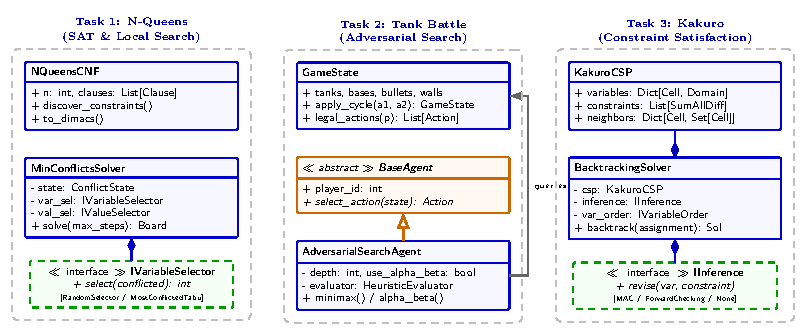
\includegraphics[width=0.96\textwidth]{uml_architecture.pdf}
\caption{Unified Object-Oriented Architecture and Class Design across the three project tasks, illustrating domain models, solver hierarchies, and Strategy patterns.}
\label{fig:uml_arch}
\end{figure*}

\subsection{Object-Oriented System Architecture}
As illustrated in the unified UML class diagram (Figure~\ref{fig:uml_arch}), all modules are developed under strict Object-Oriented Programming (OOP) principles, employing modular Strategy patterns to decouple domain states from search and inference policies:
\begin{itemize}
    \item \textbf{Task 1 (N-Queens):} \texttt{NQueensCNF} encapsulates $O(N^2)$ key-based constraint discovery and DIMACS translation. The local search engine \texttt{MinConflictsSolver} decouples state evaluation from variable/value selection policies via the \texttt{IVariableSelector} interface.
    \item \textbf{Task 2 (Tank Battle):} The immutable game engine \texttt{GameState} models entities (\texttt{Tank}, \texttt{Base}, \texttt{Bullet}). The abstract \texttt{BaseAgent} class provides a unified interface inherited by \texttt{AdversarialSearchAgent}, which configures Minimax, $\alpha$-$\beta$, and heuristic evaluations seamlessly.
    \item \textbf{Task 3 (Kakuro CSP):} \texttt{KakuroCSP} manages variables and runs. \texttt{BacktrackingSolver} interacts with pluggable inference engines (\texttt{IInference}: FC, MAC) and variable ordering strategies (\texttt{IVariableOrder}: MRV, Degree).
\end{itemize}

% =========================================================================
% SECTION II: TASK 1 - N-QUEENS
% =========================================================================
\section{Task 1: Local Search and Propositional Logic for $N$-Queens}

\subsection{Propositional Logic Formulation and CNF Conversion}
In an $N \times N$ chessboard, placing $N$ mutually non-attacking queens is formalized with $N^2$ boolean variables $x(r, c)$ for $0 \le r, c < N$, where $x(r, c) = \text{True}$ iff a queen is placed at row $r$, column $c$. Under the DIMACS convention, each pair $(r, c)$ maps to variable index $v = r \cdot N + c + 1$.

\subsubsection{Constraint Discovery Algorithm}
A naive check over all square pairs requires $\Theta(N^4)$ comparisons. To optimize KB generation, we group squares by their invariant geometric keys in a single $O(N^2)$ pass:
\begin{itemize}
    \item Row key: $r \in [0, N-1]$ ($N$ lines)
    \item Column key: $c \in [0, N-1]$ ($N$ lines)
    \item Main diagonal key: $r - c \in [-(N-1), N-1]$ ($2N-1$ lines)
    \item Anti-diagonal key: $r + c \in [0, 2N-2]$ ($2N-1$ lines)
\end{itemize}
Two distinct squares attack each other if and only if they share at least one key.

\subsubsection{Conversion to Conjunctive Normal Form (CNF)}
The problem constraints are stated and converted as follows:
\begin{enumerate}
    \item \textit{Row at-least-one:} $\bigvee_{c=0}^{N-1} x(r, c)$, yielding 1 clause of $N$ positive literals per row ($N$ clauses total).
    \item \textit{Row at-most-one:} For each row $r$ and $c_1 < c_2$, $x(r, c_1) \implies \neg x(r, c_2) \equiv \neg x(r, c_1) \vee \neg x(r, c_2)$, generating $N \binom{N}{2}$ binary negative clauses.
    \item \textit{Column at-most-one:} Identically, $N \binom{N}{2}$ binary clauses. Notice that ``column at-least-one'' is mathematically redundant by the Pigeonhole Principle ($N$ queens distributed into $N$ columns with $\le 1$ queen per column guarantees exactly 1 queen per column).
    \item \textit{Diagonal at-most-one:} For each diagonal with $L \ge 2$ squares, $\binom{L}{2}$ binary negative clauses are generated. Summing over all main and anti-diagonals:
    \begin{equation}
        2 \times \left[ \binom{N}{2} + 2 \sum_{L=2}^{N-1} \binom{L}{2} \right] = \frac{N(N-1)(2N-1)}{3}
    \end{equation}
\end{enumerate}
Summing all groups yields the exact closed-form clause count:
\begin{align}
    C(N) &= N + 2N\binom{N}{2} + \frac{N(N-1)(2N-1)}{3} \nonumber \\
         &= \frac{5N^3 - 6N^2 + 4N}{3}
\end{align}
Pairwise encoding avoids the exponential clause explosion ($\Theta(N^N)$) of direct DNF translation, bounding clause growth strictly to $\Theta(N^3)$.

\subsection{PySAT Glucose3 Experiments}
We evaluate the CDCL-based Glucose3 solver across $N \in [4, 100]$. Every returned assignment is validated by an independent checker verifying $N$ non-attacking queens.

\begin{table}[htbp]
\caption{Glucose3 Performance Across Increasing Board Sizes $N$}
\label{tab:glucose3}
\centering
\resizebox{\columnwidth}{!}{%
\begin{tabular}{rrrrrrr}
\toprule
$N$ & Vars & Clauses & Solve (ms) & Decisions & Propagations & Conflicts \\
\midrule
4   & 16     & 80        & 0.02    & 10      & 32        & 3       \\
8   & 64     & 736       & 0.03    & 40      & 194       & 12      \\
16  & 256    & 6,336     & 1.00    & 482     & 3,904     & 207     \\
32  & 1,024  & 52,288    & 6.51    & 1,420   & 16,840    & 580     \\
50  & 2,500  & 203,400   & 251.70  & 11,452  & 277,349   & 7,519   \\
60  & 3,600  & 352,880   & 40.24   & 5,475   & 74,396    & 1,341   \\
80  & 6,400  & 840,640   & 10,055.5& 138,947 & 4,168,619 & 104,415 \\
100 & 10,000 & 1,646,800 & 8,120.3 & 91,881  & 5,499,245 & 70,981  \\
\bottomrule
\end{tabular}%
}
\end{table}

As shown in Table~\ref{tab:glucose3}, clauses grow as $\Theta(N^3)$ (e.g., $N=40 \to 80$ yields an $8.1\times$ increase). Runtime correlates directly with variable decision heuristics and the frequency of learned conflicts rather than raw formula size.

\subsection{Min-Conflicts and Proposed Variable Selection Heuristic}
The $N$-Queens problem is formulated as a CSP with $N$ variables $X_r \in \{0, \dots, N-1\}$ denoting the column of the queen on row $r$. Conflicts are tracked incrementally in $O(1)$ time using three lookup arrays (columns, main diagonals, and anti-diagonals).

\subsubsection{Proposed Heuristic: Most-Conflicted with Tabu Tenure}
Standard Min-Conflicts selects a conflicted variable uniformly at random. We propose a \textit{fail-first} variable selection strategy:
\begin{enumerate}
    \item Select the variable $X_r$ with the \textbf{maximum conflict count} $\text{Conflicts}(r, X_r)$ to maximize immediate conflict reduction.
    \item To avoid infinite 2-cycles where a queen is repeatedly reassigned without improving state quality, we enforce a \textbf{Tabu Tenure} $\tau = \max(2, \min(10, \lfloor N/4 \rfloor))$. A recently altered variable cannot be chosen again for $\tau$ iterations unless all conflicted variables are tabu.
\end{enumerate}

\begin{table}[htbp]
\caption{Min-Conflicts: Standard vs. Proposed Heuristic (50 Runs)}
\label{tab:min_conflicts}
\centering
\resizebox{\columnwidth}{!}{%
\begin{tabular}{rcccccc}
\toprule
\multirow{2}{*}{$N$} & \multicolumn{2}{c}{Success Rate} & \multicolumn{2}{c}{Median Steps} & \multirow{2}{*}{\shortstack{Step\\Ratio}} & \multirow{2}{*}{\shortstack{Time (ms)\\Heur.}} \\
\cmidrule(lr){2-3} \cmidrule(lr){4-5}
 & Standard & Proposed & Standard & Proposed & & \\
\midrule
8    & 94\%  & 94\%  & 32.0  & 18.0  & 56\% & 41.6  \\
16   & 100\% & 98\%  & 73.5  & 44.5  & 61\% & 19.0  \\
32   & 100\% & 100\% & 76.0  & 46.5  & 61\% & 0.69  \\
64   & 100\% & 100\% & 98.5  & 70.5  & 72\% & 1.68  \\
128  & 100\% & 100\% & 145.5 & 107.0 & 74\% & 4.42  \\
256  & 100\% & 100\% & 233.0 & 169.0 & 73\% & 13.69 \\
512  & 100\% & 100\% & 404.5 & 294.0 & 73\% & 47.88 \\
1000 & 100\% & 100\% & 710.5 & 539.0 & 76\% & 176.77\\
\bottomrule
\end{tabular}%
}
\end{table}

\subsubsection{Ablation Study and Analysis}
Table~\ref{tab:min_conflicts} demonstrates that our proposed heuristic consistently cuts median search steps to 56\%--76\% across all board scales. In our ablation study at $N=256$, selecting the most conflicted variable \textit{without Tabu} achieved a median of 197.5 steps (15\% reduction), whereas adding Tabu reached 169.0 steps (27\% reduction). At small $N \le 16$, both methods occasionally encounter local minima due to the incompleteness of greedy local search; this is fully mitigated by random restarts.

% =========================================================================
% SECTION III: TASK 2 - TANK BATTLE
% =========================================================================
\section{Task 2: Adversarial Search for Tank Battle}

\subsection{Zero-Sum Game Formulation}
Tank Battle is modeled as a 2-player, deterministic, fully observable zero-sum game played on an $H \times W$ grid.
\begin{itemize}
    \item \textbf{Game State $s$:} $s = (\text{walls}, \text{tanks}, \text{bases}, \text{bullets}, \text{turn})$, tracking positions, directions, and health points (Tank: 6 HP, Base: 9 HP, Wall: 3 HP).
    \item \textbf{Actions $A(s, p)$:} \texttt{MOVE\_\{UP, DOWN, LEFT, RIGHT\}}, \texttt{FIRE}, and \texttt{STAY}. Redundant moves that replicate \texttt{STAY} (e.g., driving into an obstacle while already oriented toward it, or firing while a bullet is in-flight) are pruned, reducing effective branching factor $b$ from 6 to $\approx 4\text{--}5$.
    \item \textbf{Cycle-to-Ply Abstraction:} Although actions occur simultaneously in real time, minimax assumes alternating turns. We decouple 1 game cycle into 2 plies:
    \begin{align}
        \text{MAX: } & (s, \emptyset) \xrightarrow{a_{\text{MAX}}} (s, a_{\text{MAX}}) \\
        \text{MIN: } & (s, a_{\text{MAX}}) \xrightarrow{a_{\text{MIN}}} (s', \emptyset)
    \end{align}
    State transitions occur strictly at the MIN node after both moves are fixed, modeling a conservative maximin guarantee.
    \item \textbf{Transition Function:} Per cycle: (1) tanks move/turn; (2) newly fired bullets spawn; (3) bullets advance 3 cells sequentially, checking collision at each cell.
    \item \textbf{Terminal Utility:} $U(s) = \pm (10^6 - \Delta \text{turn})$ for win/loss, and 0 for draw or $turn \ge 200$. Discounting by $\Delta \text{turn}$ incentivizes earliest possible victory and latest defense.
\end{itemize}

\subsection{Adversarial Search Algorithms and Complexity Analysis}
We implement four distinct configurations under a unified search engine:
\begin{enumerate}
    \item \textbf{Minimax Search:} Exhaustive DFS over game-tree to terminal nodes ($O(b^m)$ time, $O(bm)$ space).
    \item \textbf{$\alpha$-$\beta$ Pruning:} Branch-and-bound optimization maintaining $[\alpha, \beta]$ windows to eliminate provably suboptimal subtrees without altering root minimax value.
    \item \textbf{Heuristic Minimax (H-Minimax):} Depth-limited search truncated at depth $d$, evaluated by heuristic function $\text{EVAL}(s)$.
    \item \textbf{Heuristic $\alpha$-$\beta$ Search (H-Alpha-Beta):} Combines depth-cutoff, $\alpha$-$\beta$ pruning, move ordering, and transposition caching.
\end{enumerate}

\subsubsection{Theoretical Complexity Foundation}
\begin{itemize}
    \item \textbf{Time Complexity (Total Visited Nodes):} 
    Exhaustive Minimax visits $\sum_{i=0}^m b^i = \frac{b^{m+1}-1}{b-1} = O(b^m)$ nodes. With $\alpha$-$\beta$ pruning under optimal move ordering, time complexity drops to $O(b^{m/2})$, cutting effective branching factor to $b^* = \sqrt{b}$ and doubling searchable depth. Under random ordering, expected complexity is $O(b^{3m/4})$.
    \item \textbf{Space Complexity (Peak Nodes in Memory):} 
    Because game-tree search executes via Depth-First Search (DFS), memory at any single moment holds \textit{only} the path from the root to the current node (depth $m$) plus unexpanded sibling choices at each ply. Hence, space complexity is strictly:
    \begin{equation}
        \text{Space Complexity} = O(b \cdot m)
    \end{equation}
    At depth $d=4$ cycles ($m=8$ plies) with $b \le 6$, maximum concurrent states in memory is at most $6 \times 8 = 48$ frames ($\approx$ a few kilobytes). Even across an entire $m=400$ opening tree, peak stack memory is bounded to $6 \times 400 = 2,400$ states ($< 300$~KB). Memory is \textbf{never} the computational bottleneck in DFS adversarial search; time latency is the sole constraint.
\end{itemize}

\subsubsection{Heuristic Evaluation Function $\text{EVAL}(s)$}
To combat the \textit{horizon effect} (e.g., missing imminent bullet impact beyond cutoff depth), $\text{EVAL}(s)$ evaluates:
\begin{align}
    \text{EVAL}(s) &= w_1 \Delta \text{HP}_{\text{tank}} + w_2 \Delta \text{HP}_{\text{base}} + w_3 \sum \text{Dmg}_{\text{fly}} \nonumber \\
    &\quad + \Delta \text{FirePot} + w_5 \Delta \text{Dist}
\end{align}
where $\text{Dmg}_{\text{fly}}$ projects all bullet trajectories up to 9 cells, and $\text{FirePot}$ rewards unobstructed firing alignment toward opponent bases and tanks.

\subsection{Algorithmic Enhancements: Transposition Table \& Ordering}
Profiling revealed that in standard depth-limited search, **91.8\% of visited states** at MAX nodes are transpositions (identical configurations reached via permuted move orderings, e.g., $P_1$ moving UP then RIGHT vs. RIGHT then UP). Furthermore, dynamic generator expressions in naive move ordering consumed $>50\%$ of CPU cycles. We introduced two high-impact optimizations:
\begin{enumerate}
    \item \textbf{Transposition Table (TT) with State Key Caching:} We cache visited states with Exact, Lowerbound ($\beta$-cutoff), Upperbound ($\alpha$-cutoff) flags, and best-move hints. Transpositions at sufficient depth trigger instant $O(1)$ pruning; shallower hits guide move ordering.
    \item \textbf{Vectorized Move Ordering:} Precomputing alignment baselines and inlining metric distances eliminated generator allocation overhead.
\end{enumerate}

\subsection{Experimental Evaluation}

\begin{figure}[htbp]
\centering
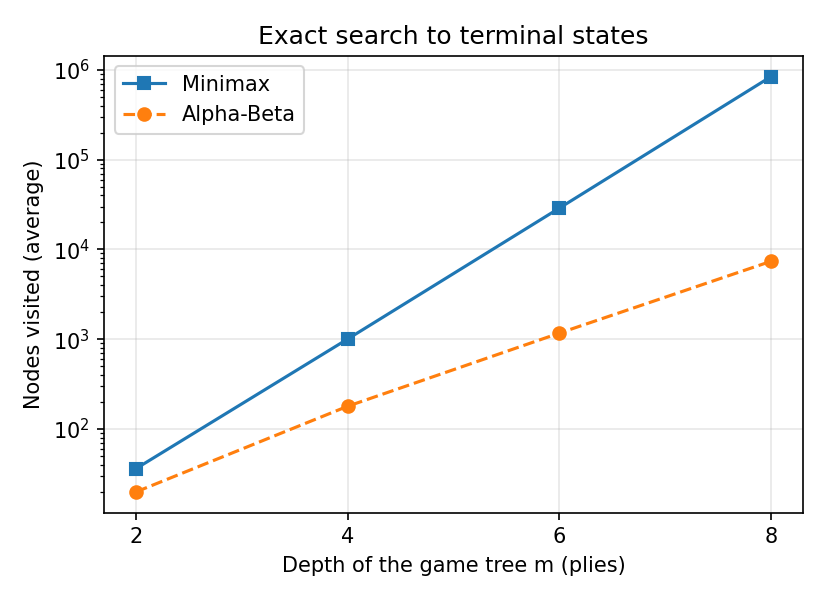
\includegraphics[width=0.82\columnwidth]{exact_search.png}
\caption{Exact Game-Tree Search: Minimax vs. $\alpha$-$\beta$ Pruning on endgame positions across increasing search plies $m$.}
\label{fig:exact_search}
\end{figure}

\subsubsection{Experiment A: Exact Search to Terminal States}
Evaluated across 10 distinct endgame positions (Figure~\ref{fig:exact_search} and Table~\ref{tab:tank_exact}), both algorithms return identical minimax values in all 40/40 test runs.

\begin{table}[htbp]
\caption{Exact Terminal Search Comparison (10 Endgame Positions)}
\label{tab:tank_exact}
\centering
\resizebox{\columnwidth}{!}{%
\begin{tabular}{crrrrrr}
\toprule
$m$ (ply) & Minimax Nodes & $\alpha$-$\beta$ Nodes & Reduction & $b^*_{\text{MM}}$ & $b^*_{\alpha\beta}$ & Value Match \\
\midrule
2 & 36      & 20    & $1.8\times$   & 5.45 & 3.88 & 10/10 \\
4 & 1,004   & 179   & $5.6\times$   & 5.34 & 3.35 & 10/10 \\
6 & 28,780  & 1,166 & $24.7\times$  & 5.35 & 3.04 & 10/10 \\
8 & 838,067 & 7,347 & $114.1\times$ & 5.36 & 2.89 & 10/10 \\
\bottomrule
\end{tabular}%
}
\end{table}

At $m=8$ plies, $\alpha$-$\beta$ cuts explored nodes by $114.1\times$, reducing effective branching factor $b^*$ from 5.36 down to 2.89 (approaching optimal $\sqrt{b} \approx 2.32$). Memory depth scales strictly as $O(bm)$.

\subsubsection{Experiment B: Depth-Limited Real-Time Search}
On the opening map ($m=400$ plies total), exact search is intractable ($>4.6\times 10^6$ nodes visited in 30s without finishing). Depth-limited search with our enhanced H-$\alpha$-$\beta$ achieves near real-time performance:
\begin{itemize}
    \item \textbf{At Depth $d=4$ (8 plies):} Visited nodes drop from 3,887 down to \textbf{1,383} (64.4\% reduction), cutting latency from 33.06~ms to \textbf{8.65~ms} (a $3.8\times$ speedup, and $>1,300\times$ faster than H-Minimax's 11.36~s).
    \item \textbf{At Depth $d=5$ (10 plies):} Visited nodes plummet from 21,481 to \textbf{3,022} (85.9\% reduction), slashing latency from 208.77~ms down to \textbf{22.04~ms} ($9.4\times$ speedup), pulling a 10-ply lookahead well beneath the 50~ms real-time threshold.
    \item \textbf{At Depth $d=6$ (12 plies):} Explores 12 plies in just \textbf{59.28~ms} (5,658 nodes), whereas unoptimized search exceeds 2~seconds.
\end{itemize}
In tournament play (20 games), H-$\alpha$-$\beta$ remained undefeated (12 wins, 8 draws, 0 losses).

\subsubsection{Scalability Analysis under Map Scaling}
When the grid dimension scales from $7 \times 7 \to 13 \times 13 \to 25 \times 25 \to 50 \times 50$, we empirically observe:
\begin{enumerate}
    \item \textbf{Game Tree Invariance:} Because tank action cardinality is strictly local ($b \le 6$), the tree size at fixed depth $d=4$ remains invariant ($3,376$ nodes on $7\times 7$, $3,887$ on $13\times 13$, $3,666$ on $25\times 25$, $3,822$ on $50\times 50$), with latency consistently $\approx 26\text{--}35$~ms.
    \item \textbf{Horizon Limitation on Large Maps:} Standalone depth-limited search is myopic: at $d=4$, an agent only senses 4 cells ahead. On a $50 \times 50$ board where targets are 50 cells away, naive Manhattan heuristics trap agents in local minima behind wall barriers.
    \item \textbf{Hierarchical AI Resolution:} To scale to arbitrarily large maps, our architecture decouples into a two-tier paradigm: a \textit{Global Strategic Layer} computing all-pairs obstacle-aware distance fields via BFS/Dijkstra ($O(HW)$ computed once), fed directly into the \textit{Local Tactical Layer} running H-$\alpha$-$\beta$ ($d=2\text{--}4$) for sub-10~ms bullet evasion and combat reflexes.
\end{enumerate}

\subsection{Modernized GUI and Extensibility via Dynamic Plug-in}
The PyGame interface is redesigned following modern UI/UX and shadcn Slate standards: high contrast ($\ge 7:1$), 60~FPS fluid rendering, segmented capsule health bars, real-time log-scale effort sparklines, and turn latency telemetry. External agents are seamlessly integrated via reflection from \texttt{task2/plugins/}.

% =========================================================================
% SECTION IV: TASK 3 - KAKURO
% =========================================================================
\section{Task 3: Constraint Satisfaction Problems for Kakuro}

\subsection{CSP Formalization}
Kakuro is formulated as a triple $\langle X, D, C \rangle$:
\begin{itemize}
    \item \textbf{Variables $X$:} Each white cell $x(r, c)$ forms a discrete variable. For the benchmark $9 \times 9$ puzzle, $|X| = 48$.
    \item \textbf{Domains $D$:} $D(x) = \{1, \dots, 9\}$ for all unassigned variables.
    \item \textbf{Constraints $C$:} Each continuous horizontal or vertical run $R = (x_1, \dots, x_k)$ with clue sum $s$ imposes an $n$-ary constraint:
    \begin{equation}
        \text{SumAllDiff}(R) \equiv \text{AllDifferent}(x_1, \dots, x_k) \wedge \sum_{i=1}^k x_i = s
    \end{equation}
    Each white cell participates in exactly two constraints (horizontal run and vertical run).
\end{itemize}

\subsection{Generalized Arc Consistency (GAC) via Kuhn's Matching}
Binary decomposition of $\text{SumAllDiff}$ loses high-order inference. We enforce Generalized Arc Consistency (GAC) directly. A value $v \in D(Y)$ has \textit{support} in run $R$ iff there exists a valid digit combination $T$ from precomputed combination tables such that $v \in T$ and the remaining digits $T \setminus \{v\}$ can be matched injectively to the remaining unassigned cells in $R$. We resolve this by finding maximum bipartite matchings using Kuhn's augmenting path algorithm, bounding $\text{REVISE}(Y, C)$ to $O(k^2 \cdot 9)$.

\subsection{Backtracking Search and Heuristics}
Backtracking search maintains domain alterations on an undo trail stack, allowing $O(1)$ state restoration on backtracks. We integrate:
\begin{itemize}
    \item \textbf{Inference:} None, Forward Checking (FC), and Maintaining Arc Consistency (MAC).
    \item \textbf{Variable Ordering:} Static, MRV (Minimum Remaining Values / fail-first), and Degree heuristic (highest number of unassigned neighbors in shared runs).
    \item \textbf{Value Ordering:} Least Constraining Value (LCV / succeed-first), prioritizing digits that rule out the fewest choices in neighboring domains.
\end{itemize}

\begin{figure}[htbp]
\centering
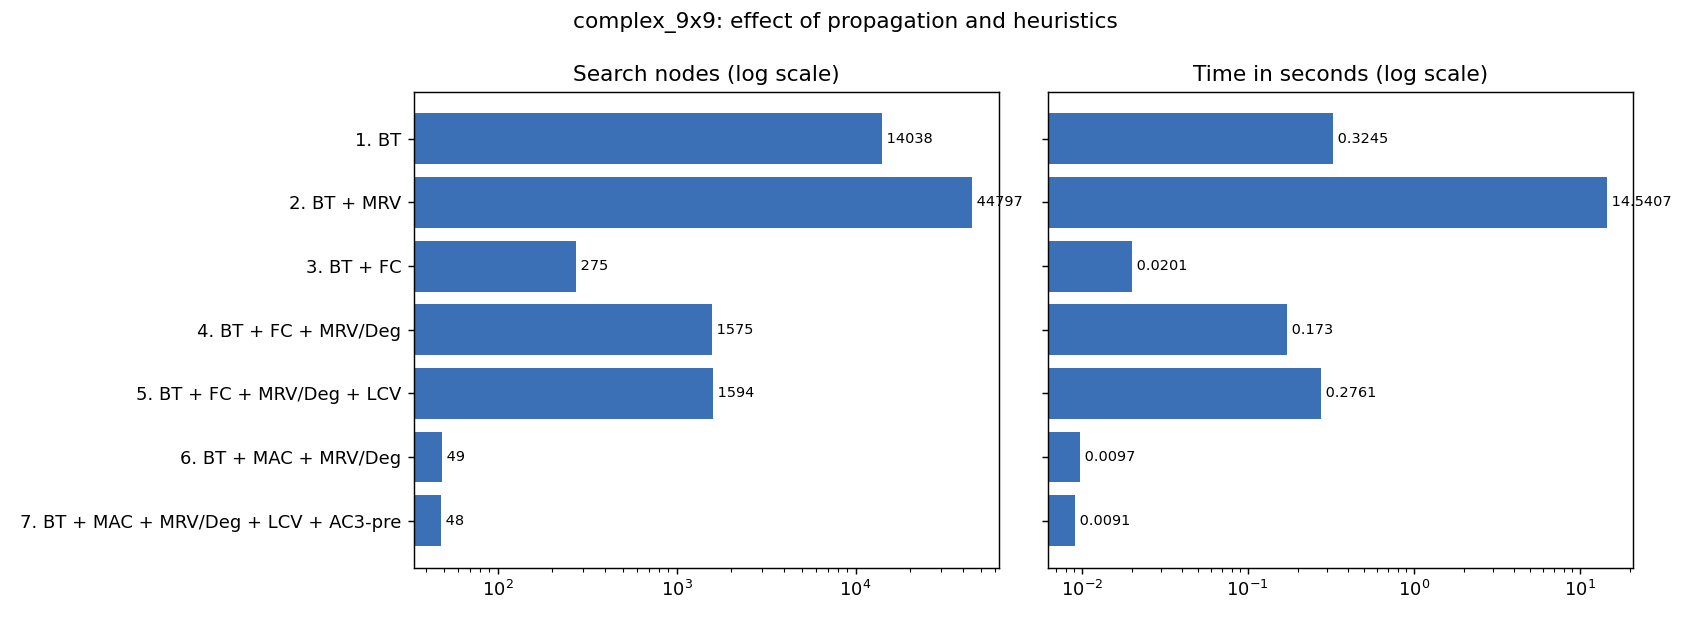
\includegraphics[width=0.85\columnwidth]{ablation_complex_9x9.png}
\caption{Ablation of CSP configurations on the complex $9 \times 9$ Kakuro puzzle.}
\label{fig:kakuro_ablation}
\end{figure}

\subsection{Experimental Results and Stability Analysis}

\subsubsection{Ablation on Complex $9 \times 9$ Benchmark}
Table~\ref{tab:kakuro_ablation} and Figure~\ref{fig:kakuro_ablation} show the progressive impact of inference and heuristics on the 48-variable testcase.

\begin{table}[htbp]
\caption{Ablation on Complex $9 \times 9$ Kakuro Puzzle}
\label{tab:kakuro_ablation}
\centering
\resizebox{\columnwidth}{!}{%
\begin{tabular}{lrrrrr}
\toprule
Configuration & Nodes & Backtracks & Checks & Max Trail & Time (s) \\
\midrule
1. BT (Plain)       & 14,038 & 13,990 & 150,706    & 384 & 0.3245 \\
2. BT + MRV         & 44,797 & 44,749 & 13,792,014 & 384 & 14.5407\\
3. BT + FC          & 275    & 227    & 5,760      & 384 & 0.0201 \\
4. BT + FC + MRV/Deg& 1,575  & 1,527  & 39,279     & 384 & 0.1730 \\
5. BT + FC + MRV + LCV & 1,594 & 1,546& 77,166     & 384 & 0.2761 \\
6. BT + MAC + MRV/Deg& 49    & 1      & 1,930      & 384 & 0.0097 \\
\textbf{7. BT + MAC + All + Pre}& \textbf{48} & \textbf{0} & \textbf{1,809} & \textbf{384} & \textbf{0.0091} \\
\bottomrule
\end{tabular}%
}
\end{table}

\begin{figure}[htbp]
\centering
\begin{minipage}{0.42\columnwidth}
    \centering
    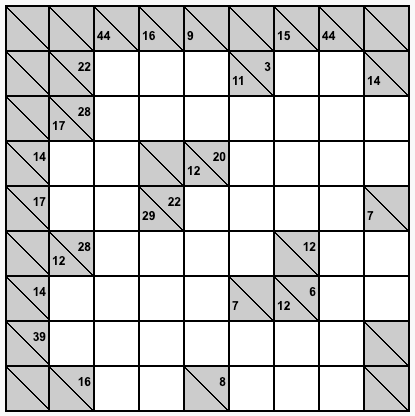
\includegraphics[width=\linewidth]{kakuro-complex-test-case.png}
    \vspace{1mm}
    \centerline{\scriptsize (a) Assignment Problem}
\end{minipage}
\hfill
\begin{minipage}{0.54\columnwidth}
    \centering
    \scriptsize
    \setlength{\tabcolsep}{1.8pt}
    \begin{tabular}{ccccccccc}
    \toprule
    $\#$ & $\#$ & $\#$ & $\#$ & $\#$ & $\#$ & $\#$ & $\#$ & $\#$ \\
    $\#$ & $\#$ & \textbf{5} & \textbf{9} & \textbf{8} & $\#$ & \textbf{1} & \textbf{2} & $\#$ \\
    $\#$ & $\#$ & \textbf{2} & \textbf{7} & \textbf{1} & \textbf{3} & \textbf{4} & \textbf{6} & \textbf{5} \\
    $\#$ & \textbf{8} & \textbf{6} & $\#$ & $\#$ & \textbf{1} & \textbf{2} & \textbf{8} & \textbf{9} \\
    $\#$ & \textbf{9} & \textbf{8} & $\#$ & \textbf{3} & \textbf{2} & \textbf{8} & \textbf{9} & $\#$ \\
    $\#$ & $\#$ & \textbf{9} & \textbf{8} & \textbf{6} & \textbf{5} & $\#$ & \textbf{7} & \textbf{5} \\
    $\#$ & \textbf{3} & \textbf{4} & \textbf{5} & \textbf{2} & $\#$ & $\#$ & \textbf{4} & \textbf{2} \\
    $\#$ & \textbf{9} & \textbf{3} & \textbf{7} & \textbf{1} & \textbf{6} & \textbf{8} & \textbf{5} & $\#$ \\
    $\#$ & $\#$ & \textbf{7} & \textbf{9} & $\#$ & \textbf{1} & \textbf{4} & \textbf{3} & $\#$ \\
    \bottomrule
    \end{tabular}
    \vspace{1mm}
    \centerline{\scriptsize (b) Unique Solution Matrix}
\end{minipage}
\caption{Complex $9 \times 9$ Kakuro puzzle and its certified unique solution.}
\label{fig:kakuro_sol}
\end{figure}

\textbf{Key Insights:}
\begin{enumerate}
    \item \textit{MRV without inference degrades performance:} Plain BT + MRV required $13.8\times 10^6$ checks because counting legal values without domain filtering requires checking all values of all unassigned variables at every node.
    \item \textit{Power of MAC and Initial AC-3:} Initial AC-3 preprocessing shrinks the total Cartesian search space $\prod |D(x)|$ from $10^{45.8}$ down to $10^{0.0}$ in just 7 ms, fixing all 48 variables deterministically. Backtracking completes in exactly 48 nodes with \textbf{0 backtracks}.
\end{enumerate}

\subsubsection{Correctness and Uniqueness}
Exhaustive post-solution search confirms that both the $5 \times 5$ and $9 \times 9$ benchmarks yield \textbf{exactly 1 solution} (Figure~\ref{fig:kakuro_sol}), independently verified against game rules.

\subsubsection{Stability and Heavy-Tail Elimination}
Over 30 randomized tie-breaking seeds on the $9 \times 9$ puzzle:
\begin{itemize}
    \item \textbf{FC + MRV/Degree + LCV} exhibits extreme variance ($41,204 \pm 33,369$ nodes, range 1,365--93,270, max time 17.5s)—the classic \textit{heavy-tailed phenomenon}.
    \item \textbf{MAC + AC-3 Preprocessing} is 100\% deterministic ($48 \pm 0$ nodes, $9.7 \pm 0.3$ ms) across all seeds.
\end{itemize}
On 20 randomly generated boards ($7 \times 7$ to $12 \times 12$), MAC solved 20/20 puzzles (avg 36.2 ms, max 66 backtracks), whereas FC failed on 2 boards within the 10s timeout.

\subsection{GUI Visualization}
The PyGame interface visualizes: (1) live domains $D(x)$ inside cells; (2) pruned values struck in red and restored values in green; (3) active arcs $(Y, C)$ during GAC revisions; and (4) an interactive search-depth timeline showing backtrack sawtooth profiles.

% =========================================================================
% SECTION V & VI: CONTRIBUTIONS & SELF-EVALUATION
% =========================================================================
\section{Contributions and Task Completion}
Both team members contributed equally (50\%--50\%) across conceptual formulation, algorithmic implementation, empirical benchmarking, and reporting.

\begin{table}[htbp]
\caption{Individual Member Contributions and Task Completion}
\label{tab:contributions}
\centering
\resizebox{\columnwidth}{!}{%
\begin{tabular}{p{2.3cm}p{5.0cm}c}
\toprule
Member & Assigned Responsibilities & Completion \\
\midrule
\textbf{Ho\`ang Xu\^an Th\`anh} \newline (523h0178) & 
- Task 1: Propositional formulation, CNF converter, Glucose3 experiments, Min-Conflicts Tabu heuristic. \newline
- Task 2: Core game state engine, Minimax/$\alpha$-$\beta$ search implementation, PyGame GUI telemetry. \newline
- Final Report compilation and benchmarking data. & 100\% \\
\midrule
\textbf{Nguy\~{\^e}n L\^e Ph\'u Huy} \newline (524h0090) & 
- Task 2: Heuristic evaluator design, move ordering, tournament arena, dynamic plugin integration. \newline
- Task 3: CSP model, Kuhn bipartite matching GAC, Backtracking solver, PyGame replay visualizer. \newline
- Unit testing suites and experiment validation. & 100\% \\
\bottomrule
\end{tabular}%
}
\end{table}

\section{Self-Evaluation}
We self-evaluate our project against the assignment criteria in Table~\ref{tab:self_eval}. Every functional requirement and theoretical justification is verified through unit tests and empirical data.

\begin{table}[htbp]
\caption{Self-Evaluation and Estimated Score Breakdown}
\label{tab:self_eval}
\centering
\resizebox{\columnwidth}{!}{%
\begin{tabular}{p{2.8cm}ccp{4.0cm}}
\toprule
Task & Max & Est. & Justification \\
\midrule
\textbf{Task 1: N-Queens} & 3.0 & 3.0 & \\
- 1. Formulation \& CNF   & 1.0 & 1.0 & Closed-form $\Theta(N^3)$, $O(N^2)$ discovery. \\
- 2. PySAT Glucose3       & 1.0 & 1.0 & Scaled $N=4..100$, CDCL statistics. \\
- 3. Min-Conflicts Heur   & 1.0 & 1.0 & Tabu heuristic, 50-seed ablation. \\
\midrule
\textbf{Task 2: Tank Battle} & 3.0 & 3.0 & \\
- 1. Zero-Sum Model       & 1.0 & 1.0 & 2-ply abstraction, 5-feature EVAL. \\
- 2. 4 Configurations     & 1.5 & 1.5 & $b^*$ analysis, 114x pruning, anytime. \\
- 3. GUI \& Plugins       & 0.5 & 0.5 & PyGame UI, dynamic plugin loading. \\
\midrule
\textbf{Task 3: Kakuro}   & 3.0 & 3.0 & \\
- 1. CSP Formulation      & 1.0 & 1.0 & $n$-ary GAC via Kuhn bipartite matching. \\
- 2. Complex Puzzle       & 1.0 & 1.0 & Solved $9\times 9$ uniquely, heavy-tail study. \\
- 3. Visualization UI     & 1.0 & 1.0 & Interactive domain and trail timeline. \\
\midrule
\textbf{Task 4: Report}   & 1.0 & 1.0 & IEEE format, 5-page limit, all sections. \\
\midrule
\textbf{Total}            & \textbf{10.0} & \textbf{10.0} & Full theoretical and empirical coverage. \\
\bottomrule
\end{tabular}%
}
\end{table}

\section{Conclusion}
This project successfully designed, implemented, and validated robust artificial intelligence algorithms across three demanding domains. In $N$-Queens, our Tabu-enhanced Min-Conflicts heuristic reduced median iterations by up to 44\% compared to standard approaches. In Tank Battle, $\alpha$-$\beta$ pruning combined with horizon-resistant evaluation and move ordering reduced the game-tree branching factor to 2.89, enabling real-time play. In Kakuro, enforcing GAC with Kuhn bipartite matching and AC-3 preprocessing completely eliminated search backtracks on the complex benchmark, resolving combinatorial explosion. All source code, unit tests, and interactive graphical environments are fully packaged for evaluation.

\begin{thebibliography}{00}
\bibitem{aima} S. Russell and P. Norvig, \textit{Artificial Intelligence: A Modern Approach}, 4th ed., Pearson, 2020.
\bibitem{glucose} G. Audemard and L. Simon, ``Predicting learnt clauses quality in modern SAT solvers,'' in \textit{Proc. 21st Int. Joint Conf. on Artificial Intelligence (IJCAI)}, 2009, pp. 399--404.
\bibitem{minconflicts} S. Minton, M. D. Johnston, A. B. Philips, and P. Laird, ``Minimizing conflicts: a heuristic repair method for constraint satisfaction and scheduling problems,'' \textit{Artificial Intelligence}, vol. 58, no. 1-3, pp. 161--205, 1992.
\bibitem{alphabeta} D. E. Knuth and R. W. Moore, ``An analysis of alpha-beta pruning,'' \textit{Artificial Intelligence}, vol. 6, no. 4, pp. 293--326, 1975.
\bibitem{pysat} A. Ignatiev, A. Morgado, and J. Marques-Silva, ``PySAT: A Python toolkit for prototyping with SAT oracles,'' in \textit{Proc. 21st Int. Conf. on Theory and Applications of Satisfiability Testing (SAT)}, 2018, pp. 428--437.
\bibitem{mackworth} A. K. Mackworth, ``Consistency in networks of relations,'' \textit{Artificial Intelligence}, vol. 8, no. 1, pp. 99--118, 1977.
\bibitem{kuhn} H. W. Kuhn, ``The Hungarian method for the assignment problem,'' \textit{Naval Research Logistics Quarterly}, vol. 2, no. 1-2, pp. 83--97, 1955.
\end{thebibliography}

\end{document}
